\documentclass[12pt,a4paper,zihao=-4,UTF8]{book}
\usepackage{lmodern}
\usepackage{amssymb,amsmath}
\usepackage{ifxetex,ifluatex}
\usepackage{fixltx2e} % provides \textsubscript
\ifnum 0\ifxetex 1\fi\ifluatex 1\fi=0 % if pdftex
  \usepackage[T1]{fontenc}
  \usepackage[utf8]{inputenc}
\else % if luatex or xelatex
  \ifxetex
    \usepackage{xltxtra,xunicode}
  \else
    \usepackage{fontspec}
  \fi
  \defaultfontfeatures{Mapping=tex-text,Scale=MatchLowercase}
  \newcommand{\euro}{€}
\fi
% use upquote if available, for straight quotes in verbatim environments
\IfFileExists{upquote.sty}{\usepackage{upquote}}{}
% use microtype if available
\IfFileExists{microtype.sty}{%
\usepackage{microtype}
\UseMicrotypeSet[protrusion]{basicmath} % disable protrusion for tt fonts
}{}
\ifxetex
  \usepackage[setpagesize=false, % page size defined by xetex
              unicode=false, % unicode breaks when used with xetex
              xetex]{hyperref}
\else
  \usepackage[unicode=true]{hyperref}
\fi
\usepackage[usenames,dvipsnames]{color}
\hypersetup{breaklinks=true,
            bookmarks=true,
            pdfauthor={},
            pdftitle={},
            colorlinks=true,
            citecolor=blue,
            urlcolor=blue,
            linkcolor=magenta,
            pdfborder={0 0 0}}
\urlstyle{same}  % don't use monospace font for urls
\usepackage{color}
\usepackage{fancyvrb}
\newcommand{\VerbBar}{|}
\newcommand{\VERB}{\Verb[commandchars=\\\{\}]}
\DefineVerbatimEnvironment{Highlighting}{Verbatim}{commandchars=\\\{\}}
% Add ',fontsize=\small' for more characters per line
\usepackage{framed}
\definecolor{shadecolor}{RGB}{248,248,248}
\newenvironment{Shaded}{\begin{snugshade}}{\end{snugshade}}
\newcommand{\KeywordTok}[1]{\textcolor[rgb]{0.13,0.29,0.53}{\textbf{#1}}}
\newcommand{\DataTypeTok}[1]{\textcolor[rgb]{0.13,0.29,0.53}{#1}}
\newcommand{\DecValTok}[1]{\textcolor[rgb]{0.00,0.00,0.81}{#1}}
\newcommand{\BaseNTok}[1]{\textcolor[rgb]{0.00,0.00,0.81}{#1}}
\newcommand{\FloatTok}[1]{\textcolor[rgb]{0.00,0.00,0.81}{#1}}
\newcommand{\ConstantTok}[1]{\textcolor[rgb]{0.00,0.00,0.00}{#1}}
\newcommand{\CharTok}[1]{\textcolor[rgb]{0.31,0.60,0.02}{#1}}
\newcommand{\SpecialCharTok}[1]{\textcolor[rgb]{0.00,0.00,0.00}{#1}}
\newcommand{\StringTok}[1]{\textcolor[rgb]{0.31,0.60,0.02}{#1}}
\newcommand{\VerbatimStringTok}[1]{\textcolor[rgb]{0.31,0.60,0.02}{#1}}
\newcommand{\SpecialStringTok}[1]{\textcolor[rgb]{0.31,0.60,0.02}{#1}}
\newcommand{\ImportTok}[1]{#1}
\newcommand{\CommentTok}[1]{\textcolor[rgb]{0.56,0.35,0.01}{\textit{#1}}}
\newcommand{\DocumentationTok}[1]{\textcolor[rgb]{0.56,0.35,0.01}{\textbf{\textit{#1}}}}
\newcommand{\AnnotationTok}[1]{\textcolor[rgb]{0.56,0.35,0.01}{\textbf{\textit{#1}}}}
\newcommand{\CommentVarTok}[1]{\textcolor[rgb]{0.56,0.35,0.01}{\textbf{\textit{#1}}}}
\newcommand{\OtherTok}[1]{\textcolor[rgb]{0.56,0.35,0.01}{#1}}
\newcommand{\FunctionTok}[1]{\textcolor[rgb]{0.00,0.00,0.00}{#1}}
\newcommand{\VariableTok}[1]{\textcolor[rgb]{0.00,0.00,0.00}{#1}}
\newcommand{\ControlFlowTok}[1]{\textcolor[rgb]{0.13,0.29,0.53}{\textbf{#1}}}
\newcommand{\OperatorTok}[1]{\textcolor[rgb]{0.81,0.36,0.00}{\textbf{#1}}}
\newcommand{\BuiltInTok}[1]{#1}
\newcommand{\ExtensionTok}[1]{#1}
\newcommand{\PreprocessorTok}[1]{\textcolor[rgb]{0.56,0.35,0.01}{\textit{#1}}}
\newcommand{\AttributeTok}[1]{\textcolor[rgb]{0.77,0.63,0.00}{#1}}
\newcommand{\RegionMarkerTok}[1]{#1}
\newcommand{\InformationTok}[1]{\textcolor[rgb]{0.56,0.35,0.01}{\textbf{\textit{#1}}}}
\newcommand{\WarningTok}[1]{\textcolor[rgb]{0.56,0.35,0.01}{\textbf{\textit{#1}}}}
\newcommand{\AlertTok}[1]{\textcolor[rgb]{0.94,0.16,0.16}{#1}}
\newcommand{\ErrorTok}[1]{\textcolor[rgb]{0.64,0.00,0.00}{\textbf{#1}}}
\newcommand{\NormalTok}[1]{#1}
\RecustomVerbatimEnvironment{Highlighting}{Verbatim}{commandchars=\\\{\},formatcom=\xeCJKVerbAddon}
\usepackage{longtable,booktabs}
\setlength{\emergencystretch}{3em}  % prevent overfull lines
\providecommand{\tightlist}{%
  \setlength{\itemsep}{0pt}\setlength{\parskip}{0pt}}
\setcounter{secnumdepth}{5}

\date{}
% !TeX document-id = {32a890c7-0db2-461b-b834-605db552d4de}
% !TEX root
% !TEX program = xelatex
% !BIB program = biber

%\def \PrintMode{} %在使用电子版论文时,请将此行注释。在打印纸质论文时,请保持本行命令不被注释,然后打印时选择双面打印即可。

%用来控制是否启动打印模式的宏,请勿改动。
\ifx \PrintMode \undefined
	\def \SideMode{oneside}
	\def \ClearPageStyle{\clearpage}
\else
	\def \SideMode{twoside}
	\def \ClearPageStyle{\cleardoublepage}
\fi

\usepackage[heading,zihao=-4]{ctex} %用来提供中文支持

\usepackage{xspace} %提供一些好用的空格命令

\usepackage{hyperref}
\hypersetup{%
	%  dvipdfmx,% 设定要使用的 driver 为 dvipdfmx
	unicode={true},% 使用 unicode 来编码 PDF 字符串
	pdfstartview={FitH},% 文档初始视图为匹配宽度
	bookmarksnumbered={true},% 书签附上章节编号
	bookmarksopen={true},% 展开书签
	pdfborder={0 0 0},% 链接无框
	citecolor=blue,
	linkcolor=blue, % blue
	anchorcolor=green,
	urlcolor=blue,
	colorlinks=true,     %注释掉此项则交叉引用为彩色边框(将colorlinks和pdfborder同时注释掉)
	pdfborder=000        %注释掉此项则交叉引用为彩色边框
	%pdfstartview=FitH,
	%pdfpagemode=FullScreen % 实现打开后全屏
}

\usepackage{cleveref} %交叉引用


%使用biblatex管理文献,输出格式使用gb7714-2015标准,后端为biber
\usepackage[backend=biber,style=gb7714-2015,hyperref=true,gbnamefmt = lowercase,gbnamefmt=familyahead, giveninits = true,maxbibnames=99]{biblatex}

%屏蔽无关的Warning
\usepackage{silence}
\WarningFilter*{biblatex}{Conflicting options.\MessageBreak'eventdate=iso' requires 'seconds=true'.\MessageBreak Setting 'seconds=true'}



%============================版面控制宏包=================================%
% 页边距:上:3.0cm,下:2.0cm,左:2.8cm,右:2.2cm,页眉:2.2cm,页脚1.5cm;
\usepackage{geometry}
\geometry{top=1.8cm,bottom=2cm,left=2.8cm,right=2.2cm,includehead,includefoot}
\usepackage[symbol,perpage]{footmisc}  % 脚注控制可使得每页的脚注编码重新复位,

\usepackage{fontspec} %设置字体需要的宏包
%设置西文字体为Times New Roman,如果没有则以开源近似字体代替
\IfFontExistsTF{Times New Roman}{
	\setmainfont{Times New Roman}
}{
	\usepackage{newtxtext,newtxmath}
}

%设置文档中文字体。优先次序:中易 > Adobe > 华文(Mac) > Fandol
\IfFontExistsTF{SimSun}{
	\setCJKmainfont[AutoFakeBold=2,ItalicFont=KaiTi]{SimSun}
}{
	\IfFontExistsTF{AdobeSongStd-Light}{
		\setCJKmainfont[AutoFakeBold=2,ItalicFont=AdobeKaitiStd-Regular]{AdobeSongStd-Light}
	}{
		\IfFontExistsTF{STSong}{
			\setCJKmainfont[AutoFakeBold=2,BoldFont=STHeiti,ItalicFont=STKaiti]{STSong}
		}{
			\setCJKmainfont[AutoFakeBold=2,BoldFont=FandolHei-Regular,ItalicFont=FandolKai-Regular]{FandolSong-Regular}
		}
	}
}
\IfFontExistsTF{SimHei}{
	\setCJKsansfont[AutoFakeBold=2]{SimHei}
}{
	\IfFontExistsTF{AdobeHeitiStd-Regular}{
		\setCJKsansfont[AutoFakeBold=2]{AdobeHeitiStd-Regular}
	}{
		\IfFontExistsTF{STHeiti}{
			\setCJKsansfont [AutoFakeBold=2]{STHeiti}
		}{
			\setCJKsansfont[AutoFakeBold=2]{FandolHei-Regular}
		}
	}
}

\renewcommand{\baselinestretch}{1.5} %1.5倍行距


\showboxdepth=5
\showboxbreadth=5


%=============================标题与列表宏包=============================%
%\usepackage{titlesec}  #             % 控制标题的宏包,配合命令在后面,
\usepackage{enumerate}              % 改变列表标号样式宏包 其后可接选项[a,A,i,I,1]
\usepackage[font=small]{caption}               % 浮动图形和表格标题样式,可选项为
% [scriptsize,footnotesize,centerlast]
\usepackage{setspace}               % 图形和表格的标题如果是多行,行距比较大,可以加宏包
%使用绝对坐标制作封面使用的宏包
\usepackage[absolute,overlay]{textpos}
\setlength{\TPHorizModule}{1mm}
\setlength{\TPVertModule}{1mm}

\usepackage{fancyvrb,shortvrb,fancyhdr}  % 支持抄录
% \usepackage{cite} % natbib不能再用了

\lhead{{\CompleteYear}年~华东师范大学学士学位论文}
\chead{}
\rhead{\TitleCHS}
\lfoot{}
\cfoot{\thepage}
\rfoot{}


%======================== 数学公式图形表格相关宏包 ===============================%
\usepackage{xcolor}
\usepackage{amsmath,amsthm,amssymb,latexsym}
\newcommand\hmmax{0} % default 3
\newcommand\bmmax{0} % default 4
\usepackage{bm}
\usepackage{mathrsfs}                % 不同于\mathcal or \mathfrak 之类的英文花体字体
\usepackage{subeqnarray}             %多个子方程(1-1a)(1-1b)
\usepackage[subnum]{cases}           % 公式环境cases
\usepackage{array,tabularx,longtable,booktabs,threeparttable,colortbl,multirow,bigstrut}
\usepackage{dcolumn}            % 让表格中将小数点对齐
\usepackage{graphicx,subfigure}
\usepackage{flafter}       % 因为图形可浮动到当前页的顶部,所以它可能会出现
% 在它所在文本的前面. 要防止这种情况,可使用 flafter宏包
\usepackage[below]{placeins}    %浮动图形控制宏包

%=========================== 特殊文本元素宏包 ==============================%
\usepackage{nicefrac}                % 在正文文本中排版分式时,可以用它来得到较好的排版效果。
\usepackage{units}                   % 基于 nicefrac 宏包,提供对计量单位比较美观的排版效果。
\usepackage{listings}                % 源代码宏包

\usepackage{makeidx}                 % 建立索引宏包
\makeindex

\pagestyle{fancy}
\setlength{\headheight}{20pt}
\hbadness=10000
\tolerance=10000

% Redefines (sub)paragraphs to behave more like sections
\ifx\paragraph\undefined\else
\let\oldparagraph\paragraph
\renewcommand{\paragraph}[1]{\oldparagraph{#1}\mbox{}}
\fi
\ifx\subparagraph\undefined\else
\let\oldsubparagraph\subparagraph
\renewcommand{\subparagraph}[1]{\oldsubparagraph{#1}\mbox{}}
\fi

\begin{document}

%%%%%%%%%%%%%%%%%%%%%%%%%%%%%%%%%%%%%%%%%%%%%%%%%%%%%%%%%%%
%
% 主文档 格式定义
%
%%%%%%%%%%%%%%%%%%%%%%%%%%%%%%%%%%%%%%%%%%%%%%%%%%%%%%%%%%%

%自定义一个空命令, 用于注释掉文本中不需要的部分.
\newcommand{\comment}[1]{}

%=============================== 脚注 =============================%
\renewcommand{\thefootnote}{\arabic{footnote}}


\allowdisplaybreaks
%\allowdisplaybreaks[n] %   n是1-4之间的数, 表示允许换页的程度,
                        %   比如\allowdisplaybreaks[0]表示可以换页但尽量不换,
                        %   而\allowdisplaybreaks[4]则是强制换页等同于\allowdisplaybreaks                        
                       
%---------------------------- 数学公式设置 ------------------------------%
\setlength{\abovedisplayskip}{2pt plus1pt minus1pt}     %公式前的距离
\setlength{\belowdisplayskip}{2pt plus1pt minus1pt}     %公式后面的距离
\setlength{\arraycolsep}{2pt}   %在一个array中列之间的空白长度, 因为原来的太宽了


%========== 目录设置 ==================================%
\setcounter{tocdepth}{2}
%\setcounter{secnumdepth}{2}
\setcounter{secnumdepth}{5}

%%%%%%%%%%%%%%%%%%%%%%%%%%%%%%%%%%%%%%%%%%%%%%%%%%%%%%%%
% 定义页眉和页脚 使用fancyhdr 宏包                     %
%%%%%%%%%%%%%%%%%%%%%%%%%%%%%%%%%%%%%%%%%%%%%%%%%%%%%%%%

\newcommand{\makeheadrule}{%
	\makebox[-3pt][l]{\rule[.7\baselineskip]{\headwidth}{0.4pt}}
	\rule[0.85\baselineskip]{\headwidth}{1.5pt}\vskip-.8\baselineskip}

\makeatletter
\renewcommand{\headrule}{%
	{\if@fancyplain\let\headrulewidth\plainheadrulewidth\fi
		\makeheadrule}}

%如果需要画单隔线, 则需要
\iffalse%-------------------------------%
\renewcommand{\headrulewidth}{0.5pt}    %在页眉下画一个0.5pt宽的分隔线
\renewcommand{\footrulewidth}{0pt}      % 在页脚不画分隔线.
\fi%------------------------------------%



%---------- 定义章节的编号格式 --------------------------%
\ctexset{chapter = {name={第,章},
				    number={\chinese{chapter}}
					}
		}
\ctexset{section = {name={\S,},
					format={\sffamily\bfseries \zihao{4}}
					}
		}
\ctexset{subsection = {name={,},
					   format={\sffamily\bfseries \zihao{-4}}
				   	}
		}
\ctexset{subsubsection = {name={,)},
     					  number={\arabic{subsubsection}},
						  format={\sffamily\bfseries \zihao{-4}},
					  	  indent = 2\ccwd 
				  	}
		}  
%\ctexset{subsubsection/runin = true}



%====================================================================%
%          中文文档定理结构的设置,重定义一些正文相关标题             %
%                    针对中文稿设置                                  %
%====================================================================%

\newtheorem{definition}{\hspace{2\ccwd}{\bf{定义}}}[chapter]
\newtheorem{proposition}{\hspace{2\ccwd}{\bf{命题}}}[chapter]
\newtheorem{property}{\hspace{2\ccwd}{\bf{性质}}}[chapter]
\newtheorem{theorem}{\hspace{2\ccwd}{\bf{定理}}}[chapter]
\newtheorem{lemma}[theorem]{\hspace{2\ccwd}{\bf{引理}}}
\newtheorem{corollary}{\hspace{2\ccwd}{\bf{推论}}}  % 需要与定理一致的编号时用此命令
\newenvironment{cor}[1][\bf{推论}]{\newline\mbox{}\hspace{2\ccwd}\textbf{#1~~~}}{\hfill $\square$ \par}
\newtheorem{axiom}{\hspace{2\ccwd}{\bf{公理}}}[chapter]
\newtheorem{exercise}{\hspace{2\ccwd}{\bf{习题}}}[chapter]
%\newtheorem{exercise}{}[chapter]
\newtheorem{question}{\hspace{2\ccwd}{\bf{问题}}}
\newtheorem{example}{\hspace{2\ccwd}{\bf{例}}}[chapter]
%\newtheorem{exam}{\hspace{2\ccwd}例}[section]
\newtheorem{notation}{\hspace{2\ccwd}{\bf{记号}}}
\newtheorem{remark}{\hspace{2\ccwd}{\bf{注记}}}
\newtheorem{assumA}{{\bf 假设A-\hspace{-1mm}}}
\newtheorem{assumB}{{\bf 假设B-\hspace{-1mm}}}

\renewenvironment{proof}[1][证明]{\textbf{#1~~~}}{\hfill $\blacksquare$}
%\renewenvironment{proof}[1][Proof]{\textbf{#1.}}{\rule{0.5em}{0.5em}}
\newenvironment{solution}[1][解]{\textbf{#1~~~}}{\hfill $\blacksquare$} %{\hfill $\square$}
%\renewenvironment{proof}[1][Proof]{\textbf{#1.}}{\rule{0.5em}{0.5em}}

%===================================================================%
%                         各种标题样式
%===================================================================%
%======================= 标题名称中文化 ============================%
\renewcommand\contentsname{目\ 录}
\renewcommand\listfigurename{插\ 图\ 目\ 录}
\renewcommand\listtablename{表\ 格\ 目\ 录}
\renewcommand\bibname{参\ 考\ 文\ 献}    %book类型
\renewcommand\indexname{索\ 引}
\renewcommand\figurename{图}
\renewcommand\tablename{表}

%========= 定制图形和表格标题样式 =====================%
\captionsetup[table]{labelsep=quad}
\captionsetup[figure]{labelsep=quad}
\captionsetup[table]{labelfont=bf,textfont={rm}}
\captionsetup[figure]{labelfont=bf,textfont={rm}}


%设置各种常用环境的交叉引用格式
\crefname{equation}{公式}{公式}
\crefname{table}{表}{表}
\crefname{figure}{图}{图}


\crefformat{theorem}{#2\bfseries{\sffamily 定理} #1#3}
\crefformat{lemma}{#2\bfseries{\sffamily 引理} #1#3}
\crefformat{corollary}{#2\bfseries{\sffamily 推论} #1#3}
\crefformat{definition}{#2\bfseries{\sffamily 定义} #1#3}
\crefformat{conjecture}{#2\bfseries{\sffamily 猜想} #1#3}
\crefformat{problem}{#2\bfseries{\sffamily 问题} #1#3}
\crefformat{proposition}{#2\bfseries{\sffamily 命题} #1#3}
\crefformat{remark}{#2\bfseries{\sffamily 注记} #1#3}
\crefformat{example}{#2\bfseries{\sffamily 例} #1#3}

\frontmatter         \sloppy            


\newcommand{\TitleCHS}{华东师范大学本科毕业论文\LaTeX 模板} %中文标题

\newcommand{\TitleENG}{\LaTeX\xspace Template for  Undergraduate Dissertation in ECNU } %英文标题

\newcommand{\Author}{~李~某~} %作者名字

\newcommand{\StudentID}{~YS012345678~} %学号

\newcommand{\Department}{~统计学院~} %学院

\newcommand{\Major}{~统计学~} %专业

\newcommand{\Supervisor}{~某某某~} %导师名字

\newcommand{\AcademicTitle}{~教授~} %导师职称

\newcommand{\CompleteDate}{~2020年5月~} %毕业年份

\newcommand{\CompleteYear}{2020} %毕业月份

\newcommand{\KeywordsCHS}{论文,模板,博士,硕士,\LaTeX,CJK, XeLaTeX } %中文关键词

\newcommand{\KeywordsENG}{thesis, template, doctor, master, \LaTeX, CJK} %英文关键词


\newgeometry{top=2.0cm, bottom=2.0cm,left=3.18cm, right=3.18cm}

%请不要修改本页的任何代码!
%请不要修改本页的任何代码!
%请不要修改本页的任何代码!
\thispagestyle{empty}
\begin{titlepage}
	\captionsetup{belowskip=0pt}
%	
\newcommand{\TitleCHS}{华东师范大学本科毕业论文\LaTeX 模板} %中文标题

\newcommand{\TitleENG}{\LaTeX\xspace Template for  Undergraduate Dissertation in ECNU } %英文标题

\newcommand{\Author}{~李~某~} %作者名字

\newcommand{\StudentID}{~YS012345678~} %学号

\newcommand{\Department}{~统计学院~} %学院

\newcommand{\Major}{~统计学~} %专业

\newcommand{\Supervisor}{~某某某~} %导师名字

\newcommand{\AcademicTitle}{~教授~} %导师职称

\newcommand{\CompleteDate}{~2020年5月~} %毕业年份

\newcommand{\CompleteYear}{2020} %毕业月份

\newcommand{\KeywordsCHS}{论文,模板,博士,硕士,\LaTeX,CJK, XeLaTeX } %中文关键词

\newcommand{\KeywordsENG}{thesis, template, doctor, master, \LaTeX, CJK} %英文关键词

	\renewcommand{\ULthickness}{1.2pt}
	\begin{center}\noindent \bfseries \zihao{4}{\rmfamily{\CompleteYear 届本科生学士学位论文\hfill 学校代码:\uline{10269}}}\end{center}
	
	\begin{textblock}{146.4}(31.8,31)
		\centering
		
\includegraphics{./figures/inner-cover(contains_font).eps}
	\end{textblock}
	
	\begin{textblock}{146.4}(31.8,125)
		\setstretch{2.0}
		\noindent
		\begin{minipage}[t][8.2cm][c]{\linewidth}
			\begin{center}
				\noindent\textbf{\zihao{2}{\rmfamily{\expandafter\expandafter{\TitleCHS}}}}
			\end{center}
			\begin{center}
				\noindent\textbf{\zihao{2}{\rmfamily{\expandafter\expandafter{\TitleENG}}}}
			\end{center}
		\end{minipage}
	\end{textblock}
	
	\renewcommand{\ULthickness}{0.4pt}
	
	\begin{textblock}{146.4}(31.8,208)
		\begin{center}
			\renewcommand{\arraystretch}{0.9}
			\bfseries\zihao{4}\rmfamily
			\begin{tabular}{ l r }
				\makebox[5\ccwd][c]{姓\hfill 名:}                   & \underline{{\makebox[5cm][c]{\Author}}}        \\
				\makebox[5\ccwd][c]{学\hfill 号:}                   & \underline{{\makebox[5cm][c]{\StudentID}}}     \\
				\makebox[5\ccwd][c]{学\hfill 院:}                   & \underline{{\makebox[5cm][c]{\Department}}}    \\
				\makebox[5\ccwd][c]{专\hfill 业:}                   & \underline{{\makebox[5cm][c]{\Major}}}         \\
				\makebox[5\ccwd][c]{指\hfill 导\hfill 教\hfill 师:} & \underline{{\makebox[5cm][c]{\Supervisor}}}    \\
				\makebox[5\ccwd][c]{职\hfill 称:}                   & \underline{{\makebox[5cm][c]{\AcademicTitle}}} \\
				\makebox[5\ccwd][c]{完\hfill 成 \hfill 时\hfill 间:} & \underline{{\makebox[5cm][c]{\CompleteDate}}} \\
			\end{tabular}\\
		\end{center}
	\end{textblock}
	
\end{titlepage}

\restoregeometry
\addtocontents{toc}{\protect\thispagestyle{empty}}

\begin{spacing}{1}
  %-------目录------------------------
\thispagestyle{empty} %取消当前页眉
%\setcounter{page}{1}

%目录中的点间距太大,改变 \@dotsep 的值可以减小
\makeatletter
    \renewcommand{\@dotsep}{0.8}
\makeatother

\newcommand{\loflabel}{图}
\newcommand{\lotlabel}{表}

\setcounter{page}{0}


\tableofcontents

% 插图目录
%\renewcommand{\numberline}[1]{\loflabel~#1\hspace*{1em}}
%\listoffigures

% 表格目录
%\renewcommand{\numberline}[1]{\lotlabel~#1\hspace*{1em}}
%\listoftables


\end{spacing}

\renewcommand{\baselinestretch}{1.8}

\chapter*{摘~~~~要}\addcontentsline{toc}{chapter}{\bf 摘要}

此模板根据CTeX上提供的清泉(吴迎年,
华北电力大学)的博/硕士论文模板(LaTeXBook2.02)和
其它类似的论文模板(如清华大学博士/硕士论文模板,袁轶君的华东师范大学本科毕业论文\TeX{}模板)修改后完成.
2013之前的版本仅适用于Windows系统, 主要为BGK编码.
2014版开始适合于所有的操作系统, 采用UTF-8编码,
且使用\XeLaTeX{}进行编译.

2020版在2014版的基础上进行了进一步改进,采用\XeLaTeX{}对正文进行编译,
用biblatex包的biber对文献进行处理和生成,文献风格采用国标GB/T4711-2015.\\
新的版本在Windows操作系统的CTeX2.9.x及Mac
OSX的MacTeX及更一般的TeXLive2019下测试通过.

一般而言,中文摘要包含500-1000字,1-2页。关键词5-10个。

\vspace{1em} \noindent  \textbf{关键词:} \rmfamily \KeywordsCHS

\renewcommand{\baselinestretch}{1.8}

\addcontentsline{toc}{chapter}{\bf ABSTRACT(英文摘要)}\chapter*{Abstract}

This template is based on Qinquan's Doctor/Master thesis template
(LaTeXBook2.02) and similar thesis templates (e.g.~Tsinghua's
Doctor/Master thesis template). It has been tested under the full
version of CTeX2.4.2 (with miktex2.4) or later.

Generally, the abstract and the key words should be consistent with the
Chinese version.

\vspace{1em} \noindent  \textbf{Key Words:} \KeywordsENG

\mainmatter 

\renewcommand{\baselinestretch}{1.5}

\fontsize{11pt}{12pt}\selectfont

\pagenumbering{arabic} \setcounter{page}{1}

\chapter{引言}

\section{引言内容}

简单介绍与论文选题有关的背景资料,包括国内外的研究现状,存在的问题,主要的参考文献,研究本文的动机,以后部分论文的基本结构。

\section{模板特色}

\begin{enumerate}
\def\labelenumi{\arabic{enumi}.}
\item
  根据华东师范大学本科毕业论文的要求定制(使用\TeX 技术)
\item
  相比于Word和\TeX 提升50-80\%的工作效率
\item
  通过Rmarkdown包实现对R, markdown, \TeX 的全面支持
\item
  免去复杂\TeX 命令, 仅通过简单的markdown标记语言实现快速写作
\item
  标准格式的pdf/高精度\TeX 输出
\item
  通过章节分类管理实现快速编译与整合
\item
  支持直接运行R和Python代码,并将生成的图形和表格嵌入到文档中
\item
  支持本地图形的插入
\item
  支持生成的R与Python图形自动添加题注(caption)
\item
  支持使用\TeX 命令对浮动公式、图形和表格进行引用
\item
  通过biblatex/biber实现对国标GB/T7714-2015格式参考文献支持
\item
  支持R代码抄录,且语法高亮显示
\item
  支持Python代码抄录,且语法高亮显示
\end{enumerate}

\section{模板使用说明}

\subsection{软件安装}

\begin{enumerate}
\def\labelenumi{\arabic{enumi}.}
\item
  \href{https://www.r-project.org/}{R3.6.2以上}
\item
  \href{https://rstudio.com/}{Rstudio}
\item
  R包: rmarkdown(支持R+markdown+TeX写作), rticles(支持ctex排版)
\item
  TeX: ctex套装(仅适用于Windows) 或 TeXLive2019(推荐, 适用于Windows,
  MacOS, Linux) 或 TinyTeX(适用于Windows, MacOS)
\end{enumerate}

\subsection{TinyTeX的安装}\label{tinytex}

\begin{enumerate}
\def\labelenumi{\arabic{enumi}.}
\item
  说明:
  TinyTeX是谢益辉开发的微型TeXLive套件,适合于对数学公式要求不要的\TeX{}软件用户,
  运行过程中对于缺省的\TeX{}包可通过tlmgr实现自动在线安装。
\item
  安装 tinytex R包
\end{enumerate}

\begin{itemize}
\tightlist
\item
  CRAN安装
\end{itemize}

\begin{Shaded}
\begin{Highlighting}[]
\KeywordTok{install.packages}\NormalTok{(}\StringTok{'tinytex'}\NormalTok{)}
\end{Highlighting}
\end{Shaded}

\begin{itemize}
\tightlist
\item
  github安装
\end{itemize}

\begin{Shaded}
\begin{Highlighting}[]
\NormalTok{devtools}\OperatorTok{::}\KeywordTok{install_github}\NormalTok{(}\StringTok{'yihui/tinytex'}\NormalTok{)}
\NormalTok{tinytex}\OperatorTok{::}\KeywordTok{install_tinytex}\NormalTok{()}
\end{Highlighting}
\end{Shaded}

\begin{enumerate}
\def\labelenumi{\arabic{enumi}.}
\setcounter{enumi}{1}
\tightlist
\item
  安装TinyTeX
\end{enumerate}

\begin{Shaded}
\begin{Highlighting}[]
\NormalTok{tinytex}\OperatorTok{::}\KeywordTok{install_tinytex}\NormalTok{()}
\end{Highlighting}
\end{Shaded}

\begin{enumerate}
\def\labelenumi{\arabic{enumi}.}
\setcounter{enumi}{2}
\tightlist
\item
  卸载TinyTeX
\end{enumerate}

\begin{Shaded}
\begin{Highlighting}[]
\NormalTok{tinytex}\OperatorTok{::}\KeywordTok{uninstall_tinytex}\NormalTok{()}
\end{Highlighting}
\end{Shaded}

\chapter{论文构成}

毕业论文格式应规范,必须由封面、目录、正文(包括中外文题名、中外文摘要、中外文关键词、正文、参考文献和致谢)三部分构成。论文装订顺序为

\begin{itemize}
\item
  外封面
\item
  开题报告
\item
  内封面
\item
  目录
\item
  中文摘要: 中文题名,中文摘要内容,中文关键词
\item
  英文摘要: 英文题名, 英文摘要内容, 英文关键词
\item
  正文
\item
  参考文献(至少包含二篇英文文献)
\item
  附录
\item
  致谢
\item
  考核意见表
\end{itemize}

\chapter{正文要求}

\section{基本要求}

\subsection{字数要求}

5000字以上.

\subsection{封面要求}

\subsubsection{要求1}\label{1}

上交的每份论文都一律采用学校统一印发的外封面(装订线一律在左面)。

\subsubsection{要求2}\label{2}

另附自制内封面一份(A4纸张电脑打印),内容为中外文论文题目、作者的姓名、学号、班级、指导老师的姓名与职称、论文完成时间。

\subsection{纸张及装订要求}

毕业论文一律用A4纸张电脑打印。左侧装订。

\subsection{开题报告要求}

开题报告内容包括:选题的背景与意义(对与选题有关的国内外研究现状、进展情况、存在的问题等进行调研,在此基础上提出选题的研究意义),课题研究的主要内容、方法、技术路线,课题研究拟解决的主要问题及创新之处,课题研究的总体安排与进度,参考文献等方面。开题报告表格至教务处网站下载。

\section{有序列表}

\begin{enumerate}
\def\labelenumi{\arabic{enumi}.}
\item
  项目列表
\item
  项目列表
\item
  项目列表

  \begin{enumerate}
  \def\labelenumii{\alph{enumii}.}
  \item
    项目列表
  \item
    项目列表
  \item
    项目列表
  \end{enumerate}
\end{enumerate}

\section{无序列表}

\begin{itemize}
\item
  项目列表
\item
  项目列表

  \begin{itemize}
  \item
    项目列表
  \item
    项目列表
  \item
    项目列表
  \end{itemize}
\end{itemize}

\section{公式}

\subsection{单行公式}

\begin{itemize}
\item
  公式示例1: \[\mu_1\le\mu_2\le \dots\le \mu_k.\]
\item
  公式示例2:

  \begin{equation}\label{eq1}
    x^2+y^2=1
  \end{equation}
\item
  引用: 公式\eqref{eq1}或使用cleveref包,\cref{eq1}.
\end{itemize}

\subsection{多行公式}

\begin{itemize}
\item
  公式示例3:\\

  \begin{align}
    x^2+y^2 &= 1 \label{eq4}\\
    x_2+y_2 &= 0  \label{eq5}
  \end{align}
\item
  引用: \cref{eq4}和\cref{eq5}
\item
  公式示例4:\\
  \[
  f(x)=\begin{cases} 1, & \mbox{If $x\ge 0$}, \\ 0,& \mbox{Otherwise,}\end{cases}
  \]
\item
  公式示例5:\\

  \begin{numcases}{|x|=}
  x, & for $x \geq 0$\\
  -x, & for $x < 0$
  \end{numcases}
\end{itemize}

\section{插入图形}

\subsection{插入R产生的图形}\label{r}

\begin{itemize}
\tightlist
\item
  图形示例1: R图\ref{fig:Rfig-1}或使用cleveref包,\cref{fig:Rfig-1}
\end{itemize}

\begin{figure}[h]

{\centering 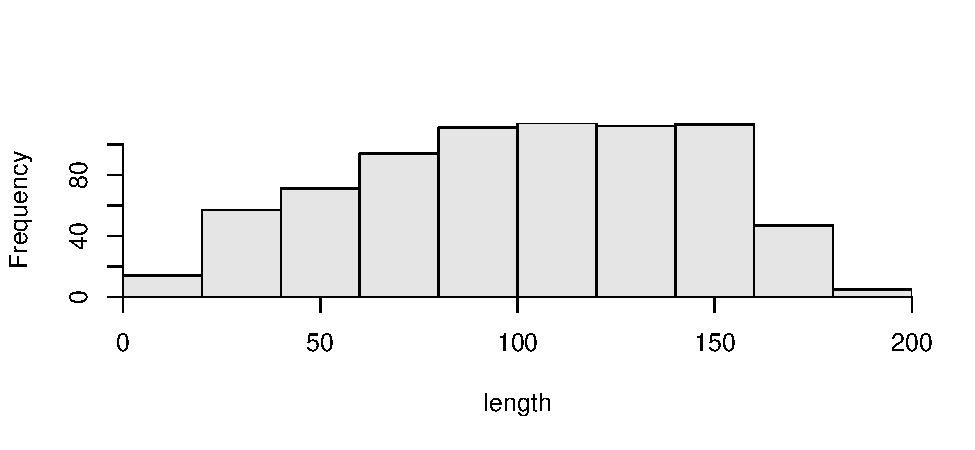
\includegraphics[width=0.7\linewidth]{figures/unnamed-chunk-10-1} 

}

\caption{\label{fig:Rfig-1}1992年捕获的Ruffe的长度的频数.\protect\linebreak Figure\ref{fig:Rfig-1} Length frequency of captured ruffes in 1992.}\label{fig:unnamed-chunk-10}
\end{figure}

\subsection{插入本地图形}

\begin{itemize}
\tightlist
\item
  本地图形: \cref{fig:local-fig}.
\end{itemize}

\begin{figure}[h]

{\centering 
\includegraphics[width=0.7\linewidth]{figures/example-image} 

}

\caption{\label{fig:local-fig}插入本地图形.\protect\linebreak Figure \ref{fig:local-fig}  Insert a local figure.}\label{fig:locfig}
\end{figure}

\section{插入表格}

\subsection{插入R生成的表格}\label{r}

\begin{itemize}
\tightlist
\item
  R产生的数据列表
\end{itemize}

\begin{Shaded}
\begin{Highlighting}[]
\KeywordTok{summary}\NormalTok{(cars)}
\end{Highlighting}
\end{Shaded}

\begin{verbatim}
     speed           dist       
 Min.   : 4.0   Min.   :  2.00  
 1st Qu.:12.0   1st Qu.: 26.00  
 Median :15.0   Median : 36.00  
 Mean   :15.4   Mean   : 42.98  
 3rd Qu.:19.0   3rd Qu.: 56.00  
 Max.   :25.0   Max.   :120.00  
\end{verbatim}

\subsection{\texorpdfstring{使用\texttt{xtable}:
\cref{tab:xtable}}{使用xtable: }}\label{xtable}

\begin{table}[ht]
\centering
\caption{\label{tab:xtable}Iris数据-xtable.\protect\linebreak Table\ref{tab:xtable}   Iris data-xtable} 
\begin{tabular}{rrrrrl}
  \hline
 & Sepal.Length & Sepal.Width & Petal.Length & Petal.Width & Species \\ 
  \hline
1 & 5.10 & 3.50 & 1.40 & 0.20 & setosa \\ 
  2 & 4.90 & 3.00 & 1.40 & 0.20 & setosa \\ 
  3 & 4.70 & 3.20 & 1.30 & 0.20 & setosa \\ 
  4 & 4.60 & 3.10 & 1.50 & 0.20 & setosa \\ 
  5 & 5.00 & 3.60 & 1.40 & 0.20 & setosa \\ 
  6 & 5.40 & 3.90 & 1.70 & 0.40 & setosa \\ 
   \hline
\end{tabular}
\end{table}

\subsection{\texorpdfstring{使用 Kable:
\cref{tab:kable1}}{使用 Kable: }}\label{-kable}

\begin{Shaded}
\begin{Highlighting}[]
\NormalTok{n <-}\StringTok{ }\DecValTok{100}
\NormalTok{x <-}\StringTok{ }\KeywordTok{rnorm}\NormalTok{(n)}
\NormalTok{y <-}\StringTok{ }\DecValTok{2}\OperatorTok{*}\NormalTok{x }\OperatorTok{+}\StringTok{ }\KeywordTok{rnorm}\NormalTok{(n)}
\NormalTok{out <-}\StringTok{ }\KeywordTok{lm}\NormalTok{(y }\OperatorTok{~}\StringTok{ }\NormalTok{x)}
\KeywordTok{library}\NormalTok{(knitr)}
\KeywordTok{kable}\NormalTok{(}\DataTypeTok{caption =} \StringTok{"}\CharTok{\textbackslash{}\textbackslash{}}\StringTok{label\{tab:kable1\}kable表.}\CharTok{\textbackslash{}\textbackslash{}}\StringTok{protect}\CharTok{\textbackslash{}\textbackslash{}}\StringTok{linebreak  Table}\CharTok{\textbackslash{}\textbackslash{}}\StringTok{ref\{tab:kable1\}\textbackslash{} \textbackslash{} Table with kable."}\NormalTok{, }
      \KeywordTok{summary}\NormalTok{(out)}\OperatorTok{$}\NormalTok{coef, }\DataTypeTok{digits=}\DecValTok{2}\NormalTok{,  }\DataTypeTok{booktabs=}\OtherTok{TRUE}\NormalTok{)}
\end{Highlighting}
\end{Shaded}

\begin{longtable}[]{@{}lrrrr@{}}
\caption{\label{tab:kable1}kable表.\protect\linebreak  Table\ref{tab:kable1}
Table with kable.}\tabularnewline
\toprule
& Estimate & Std. Error & t value &
Pr(\textgreater{}\textbar{}t\textbar{})\tabularnewline
\midrule
\endfirsthead
\toprule
& Estimate & Std. Error & t value &
Pr(\textgreater{}\textbar{}t\textbar{})\tabularnewline
\midrule
\endhead
(Intercept) & -0.08 & 0.1 & -0.87 & 0.39\tabularnewline
x & 1.94 & 0.1 & 19.53 & 0.00\tabularnewline
\bottomrule
\end{longtable}

\subsection{\texorpdfstring{使用 Kable---带脚注:
\cref{tab:kable2}}{使用 Kable---带脚注: }}\label{-kable}

\begin{table}[t]

\caption{\label{tab:unnamed-chunk-12}\label{tab:kable2}mtcars数据-带脚注.\protect\linebreak Table\ref{tab:kable2}  Data of mtcars with footenote.}
\centering
\begin{tabular}{l|r|r|r|r}
\hline
\multicolumn{1}{c|}{ } & \multicolumn{2}{c|}{Group 1} & \multicolumn{2}{c}{Group 2\textsuperscript{a}} \\
\cline{2-3} \cline{4-5}
  & mpg & cyl & disp & hp\\
\hline
Mazda RX4 & 21.0 & 6 & 160 & 110\\
\hline
Mazda RX4 Wag & 21.0 & 6 & 160 & 110\\
\hline
Datsun 710 & 22.8 & 4 & 108 & 93\\
\hline
Hornet 4 Drive & 21.4 & 6 & 258 & 110\\
\hline
Hornet Sportabout & 18.7 & 8 & 360 & 175\\
\hline
\multicolumn{5}{l}{\textsuperscript{a} table footnote}\\
\end{tabular}
\end{table}

\newcommand{\bbb}{这是一个针对定理类环境进行的科技文稿排版测试}

\section{定理型环境示例}

\begin{definition} 
\bbb
\end{definition}

\begin{theorem}\label{th1}
 \bbb
\end{theorem}

\begin{proof}
\bbb
\end{proof}

\begin{corollary}\label{cor1}
\bbb
\end{corollary}

\begin{lemma}\label{lem1}
\bbb
\end{lemma}

\begin{example}
\bbb
\end{example}

\section{脚注与引用}

\subsection{脚注}

这里是脚注测试\footnote{1111111111}这里是脚注测试这里是脚注测试这里是脚注测试\footnote{2222222222}这里是脚注测试这里是脚注测试这里是脚注测试这里是脚注测试这里是脚注测试这里是脚注测试这里是脚注测试这里是脚注测试这里是脚注测试这里是脚注测试这里是脚注测试这里是脚注测试这里是脚注测试这里是脚注测试这里是脚注测试\footnote{3333333333}这里是脚注测试这里是脚注测试这里是脚注测试这里是脚注测试这里是脚注测试这里是脚注测试这里是脚注测试这里是脚注测试这里是脚注测试这里是脚注测试这里是脚注测试这里是脚注测试

\subsection{定理类引用}

由\cref{th1}我们可以知道XXXXXXXX。

由\cref{lem1}我们可以知道XXXXXXXX。

由\cref{cor1}我们可以知道XXXXXXXX。

\subsection{文献引用的演示}

本模板使用biblatex进行文献管理,这是一套相对较新的系统。另外,使用了hushidong制作的符合gb7714-2015标准的biblatex样式。在此对他的工作表示感谢,要完成这样的样式非常不容易。本模板中gb7714-2015.bbx与gb7714-2015.cbx即为他的作品,在这里打包发布以便使用。详见\url{https://github.com/hushidong/biblatex-gb7714-2015}查找相关资料。

默认的bib文件位于\textasciitilde{}/reference/thesis-ref.bib,内容是由Wang
Tianshu制作。文献库\textasciitilde{}/reference/refs.bib收集了一些典型的例子,在此仅作演示之用。
关于bib文件的编写与管理请自行查找相关教程。

例如文献\cite{Xiedy:1997}是最早介绍\TeX{}的中文参考书。

\nocite{*}

\chapter{总结与展望}

概要回顾论文的主要结论,并提出一些展望。

本论文提供了一个完整的华东师范大学本科毕业论文模板. 这套模板符合
学校的有关要求, 方便易用. 这一工作对广大研究生更好地撰写学位论文无疑
带来很大的便利, 在其它场合同样会发挥重要的作用.

\phantomsection
\addcontentsline{toc}{chapter}{\bf 参考文献}
\printbibliography[title={\centerline{\bfseries\sffamily \zihao {-3}参考文献}}]

\begin{appendix}
    \renewcommand{\chaptername}{附录 \Alph{chapter}}
    \renewcommand{\thesection}{\Alph{chapter}.\arabic{section}}
    \renewcommand{\thesubsection}{\Alph{chapter}.\arabic{section}.\arabic{subsection}}
    \renewcommand{\thesubsubsection}{\arabic{subsubsection}.}
    \renewcommand{\thetable}{\Alph{chapter}-\arabic{table}}
    \renewcommand{\theequation}{\Alph{chapter}-\arabic{equation}}
    \renewcommand{\thefigure}{\Alph{chapter}-\arabic{figure}}
\end{appendix}

\chapter{附录标题}

加油! 终于到最后一个部分了!

\section{附录中的图形、表格、公式}

附录中的公式(\ref{equ:Call})和(\ref{equ:Put})分别为:

\begin{equation}\label{equ:Call}
  c=S_0N(d_1)-X e^{-r T}N(d_2)
\end{equation}

和

\begin{equation}\label{equ:Put}
  p=X e^{-r T}N(-d_2)-S_0N(-d_1),
\end{equation}

\section{R代码}

\begin{itemize}
\tightlist
\item
  线性回归
\end{itemize}

\begin{Shaded}
\begin{Highlighting}[]
\KeywordTok{par}\NormalTok{(}\DataTypeTok{mar =} \KeywordTok{c}\NormalTok{(}\DecValTok{4}\NormalTok{, }\DecValTok{4}\NormalTok{, }\DecValTok{1}\NormalTok{, .}\DecValTok{1}\NormalTok{))}
\NormalTok{fit =}\StringTok{ }\KeywordTok{lm}\NormalTok{(dist }\OperatorTok{~}\StringTok{ }\DecValTok{1} \OperatorTok{+}\StringTok{ }\NormalTok{speed, }\DataTypeTok{data =}\NormalTok{ cars)}
\KeywordTok{plot}\NormalTok{(cars, }\DataTypeTok{pch =} \DecValTok{19}\NormalTok{, }\DataTypeTok{col =} \StringTok{'blue'}\NormalTok{, }\DataTypeTok{las =} \DecValTok{1}\NormalTok{)}
\KeywordTok{abline}\NormalTok{(fit, }\DataTypeTok{lwd =} \DecValTok{2}\NormalTok{)}
\end{Highlighting}
\end{Shaded}

\begin{itemize}
\tightlist
\item
  ggplot2
\end{itemize}

\begin{Shaded}
\begin{Highlighting}[]
\KeywordTok{par}\NormalTok{(}\DataTypeTok{mar =} \KeywordTok{c}\NormalTok{(}\DecValTok{4}\NormalTok{, }\DecValTok{4}\NormalTok{, }\DecValTok{1}\NormalTok{, .}\DecValTok{1}\NormalTok{))}
\NormalTok{fit =}\StringTok{ }\KeywordTok{lm}\NormalTok{(dist }\OperatorTok{~}\StringTok{ }\DecValTok{1} \OperatorTok{+}\StringTok{ }\NormalTok{speed, }\DataTypeTok{data =}\NormalTok{ cars)}
\KeywordTok{plot}\NormalTok{(cars, }\DataTypeTok{pch =} \DecValTok{19}\NormalTok{, }\DataTypeTok{col =} \StringTok{'blue'}\NormalTok{, }\DataTypeTok{las =} \DecValTok{1}\NormalTok{)}
\KeywordTok{abline}\NormalTok{(fit, }\DataTypeTok{lwd =} \DecValTok{2}\NormalTok{)}
\end{Highlighting}
\end{Shaded}

\section{Python代码}

\begin{Shaded}
\begin{Highlighting}[]
\ImportTok{import}\NormalTok{ matplotlib.pyplot }\ImportTok{as}\NormalTok{ plt}
\ImportTok{import}\NormalTok{ numpy }\ImportTok{as}\NormalTok{ np}
\NormalTok{x }\OperatorTok{=}\NormalTok{ np.arange(}\FloatTok{0.0}\NormalTok{, }\FloatTok{6.0}\NormalTok{, }\FloatTok{0.01}\NormalTok{)}
\NormalTok{plt.plot(x, [x}\OperatorTok{**}\DecValTok{2} \ControlFlowTok{for}\NormalTok{ x }\KeywordTok{in}\NormalTok{ x])}
\NormalTok{plt.show()}
\end{Highlighting}
\end{Shaded}

\backmatter 

\renewcommand{\baselinestretch}{1.8}

\chapter*{致~~~~谢}\markboth{致谢}{致谢}\addcontentsline{toc}{chapter}{\bf 致谢}

从20xx年9月至今的三年学习期间得到了统计学院许多老师、同学和朋友的帮助,
在此一并表示感谢.

在论文的选题到完成的各个阶段, 自始自终得到了导师 xxx 的细心指导和帮助,
并提供了许多宝贵的资料和建议,
其\ldots{}\ldots{}和严谨的治学精神是我整整三年学习期间最为珍贵的养份,
在此我想由忠地说一声:谢谢 xxx 老师, 谢谢你给我的无私的帮助!

最后, 也是最为重要的, 我的 xxx 多年来一直支持我的学习和研究,
在论文的完成过程中付出了大量的时间和心血. 感激之情, 难以言表,
我将永身不忘.

\clearpage

\end{document}
